\begin{frame}{El MFMP proyecta superávit primario desde 2028}
\centering
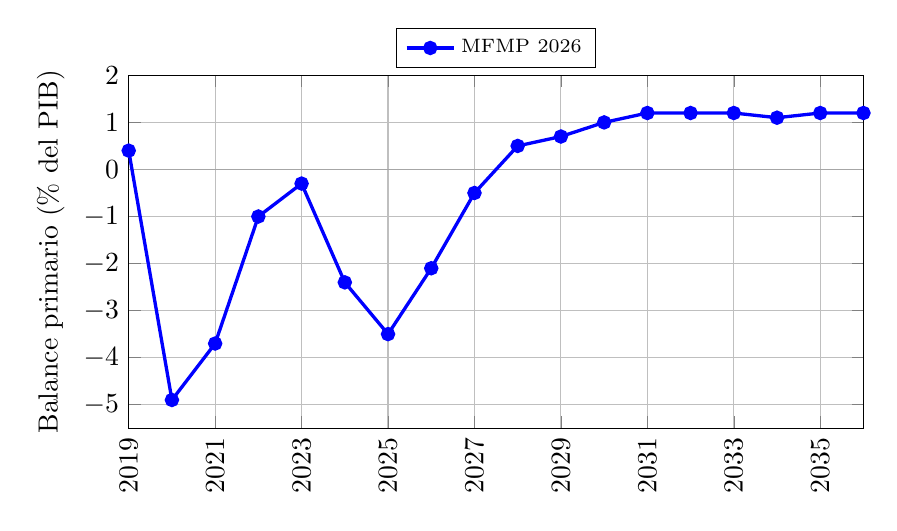
\begin{tikzpicture}
\begin{axis}[
  width=0.90\textwidth,height=0.50\textwidth,
  ylabel={Balance primario (\% del PIB)},xmin=2019,xmax=2036,ymin=-5.5,ymax=2,
  xtick={2019,2021,...,2035},xticklabel style={rotate=90,anchor=east,/pgf/number format/.cd,1000 sep={},fixed,precision=0},scaled x ticks=false,
  ytick={-5,-4,...,2},grid=both,
  legend style={at={(0.5,1.02)},anchor=south,font=\scriptsize}
]
\addplot[color=black!35,thin,forget plot] coordinates {(2019,0) (2036,0)};
\addplot[color=blue,very thick,mark=*] coordinates {
 (2019,0.4) (2020,-4.9) (2021,-3.7) (2022,-1.0) (2023,-0.3) (2024,-2.4)
 (2025,-3.5) (2026,-2.1) (2027,-0.5) (2028,0.5) (2029,0.7) (2030,1.0)
 (2031,1.2) (2032,1.2) (2033,1.2) (2034,1.1) (2035,1.2) (2036,1.2)
};
\addlegendentry{MFMP 2026}
\end{axis}
\end{tikzpicture}

\scriptsize Fuente: MFMP 2026, capítulo 3, tabla 3.1; serie histórica 2019--2024: MHCP, como en la versión fuente.
\end{frame}